% =====================================================================
%  Workshop 3 - Silver-to-Gold Pipeline Report (IEEE conference layout)
%  Team 4 - Tropical Cyclone Monitoring
%  Data Analysis Programming 2026-II, Universidad Distrital FJC
%  Build: pdflatex workshop3_report.tex (run twice)
% =====================================================================
\documentclass[10pt,twocolumn,letterpaper]{article}

% ---------- page geometry (IEEE conference, US letter) --------------
\usepackage[letterpaper,top=0.75in,bottom=1in,left=0.625in,right=0.625in,columnsep=0.25in]{geometry}
\usepackage[T1]{fontenc}
\usepackage[utf8]{inputenc}
\usepackage{mathptmx}            % Times text and math
\usepackage[scaled=0.86]{helvet}
\usepackage{courier}
\usepackage{microtype}
\usepackage{amsmath}
\usepackage{graphicx}
\usepackage{array,booktabs,tabularx,multirow,makecell}
\usepackage{stfloats}            % bottom-placed double-column floats
\usepackage{balance}
\usepackage[hyphens]{url}
\makeatletter\g@addto@macro\UrlBreaks{\do\_\do\&\do\=\do\?\do\.}\makeatother
\usepackage[colorlinks=false,pdfborder={0 0 0},pdftitle={TC-Analog Monitor: Silver-to-Gold Pipeline, Governance KPIs and Storytelling},pdfauthor={O. Pena, R. Lopez, B. Ramirez}]{hyperref}
\usepackage{listings}
\usepackage{xcolor}
\usepackage{titlesec}
\usepackage[font=footnotesize,labelsep=period]{caption}
\usepackage{enumitem}

% ---------- editable values ----------------------------------------
\newcommand{\repourl}{\url{https://github.com/Estebxnnnn/Data_Analysis_Programming}}

% ---------- IEEE-like headings --------------------------------------
\renewcommand{\thesection}{\Roman{section}}
\renewcommand{\thesubsection}{\Alph{subsection}}
\renewcommand{\thesubsubsection}{\arabic{subsubsection})}
\titleformat{\section}{\centering\normalsize\scshape}{\thesection.}{0.5em}{}
\titlespacing*{\section}{0pt}{10pt plus 2pt minus 2pt}{5pt plus 1pt}
\titleformat{\subsection}{\normalsize\itshape}{\thesubsection.}{0.5em}{}
\titlespacing*{\subsection}{0pt}{7pt plus 2pt minus 1pt}{3pt plus 1pt}
\titleformat{\subsubsection}[runin]{\normalsize\itshape}{\thesubsubsection}{0.4em}{}[:]
\titlespacing*{\subsubsection}{\parindent}{3pt}{0.5em}

% ---------- captions: "Fig. 1." below, "TABLE I" above ---------------
\renewcommand{\figurename}{Fig.}
\renewcommand{\thetable}{\Roman{table}}
\DeclareCaptionFormat{ieeetable}{\centering\textsc{#1}\\\textsc{#3}\par}
\DeclareCaptionLabelSeparator{ieeenone}{}
\captionsetup[table]{format=ieeetable,labelsep=ieeenone,skip=3pt,font=footnotesize,name=TABLE}
\captionsetup[figure]{skip=4pt,justification=justified,singlelinecheck=true}

% ---------- misc ----------------------------------------------------
\setlength{\parindent}{1em}
\setlist{nosep,leftmargin=1.4em}
\newcommand{\code}[1]{\texttt{\footnotesize #1}}
\renewcommand{\arraystretch}{1.12}
\setlength{\tabcolsep}{3.5pt}
\newcolumntype{L}[1]{>{\raggedright\arraybackslash}p{#1}}
\newcolumntype{Y}{>{\raggedright\arraybackslash}X}
\lstset{basicstyle=\ttfamily\scriptsize,breaklines=true,breakatwhitespace=false,
        columns=fullflexible,keepspaces=true,frame=tb,framerule=0.4pt,
        xleftmargin=2pt,xrightmargin=2pt,aboveskip=4pt,belowskip=4pt,
        literate={°}{{$^\circ$}}1}
\pagestyle{empty}
\renewcommand{\lstlistingname}{Listing}
\captionsetup[lstlisting]{font=footnotesize,labelsep=period,justification=centering,singlelinecheck=false,skip=2pt}
\urlstyle{same}

\begin{document}

\twocolumn[{%
\begin{center}
{\fontsize{22}{26}\selectfont TC-Analog Monitor: Silver-to-Gold Pipeline,\\[2pt] Governance KPIs and Storytelling with Historical Analogs\par}
\vspace{6pt}
{\small Data Analysis Programming, Semester 2026-II \textendash{} Workshop No.~3 (Silver-to-Gold Pipeline, Governance KPIs and Storytelling Definition)\par}
\vspace{10pt}
\begin{tabular}{@{}c@{\hspace{3.2em}}c@{\hspace{3.2em}}c@{}}
\textit{Omar Peña} & \textit{Rosa López} & \textit{Brayan Ramírez}\\
\footnotesize Student ID 20222020108 & \footnotesize Student ID 20222020134 & \footnotesize Student ID 20222020139
\end{tabular}\\[4pt]
{\footnotesize Computer Engineering Program, School of Engineering, Universidad Distrital Francisco José de Caldas, Bogotá, Colombia\\
Team 4 \textendash{} Instructor: Eng. Carlos Andrés Sierra, M.Sc. \textendash{} November 20, 2026 \textendash{} Repository: \repourl{} (branch \code{workshop-3})\par}
\vspace{12pt}
\end{center}
}]

\noindent{\bfseries\itshape Abstract}\textbf{\textemdash This report closes the medallion architecture of TC-Analog Monitor. We first audited five days of Bronze and Silver data produced by the Workshop~2 pipeline and found nine data-quality problems, among them five HTTP~400 timeouts of the GDACS API, eleven identical copies of the IBTrACS ACTIVE file, seven empty Silver files and an outlier rule that flagged the real peak of a typhoon. Each problem was fixed and measured again: IBTrACS answered ``not modified'' in 15 of 17 checks, the median delay between file timestamp and ingestion fell from about 60~min to 1.2~min, and no empty Silver file was written. A new Gold DAG reads the whole Silver folder with PySpark in local mode and produces two tidy Parquet tables: 149 governance KPI values over eight quality dimensions, and a storytelling table that compares every current storm with its five most similar storms since 1980 using the Storm Analog Similarity defined in Workshop~1. For Hurricane XAVIER the best analog scores only 29/100, which shows how unusual the storm is; for AKVAN four of five analogs reached land within 72~h.}

\vspace{4pt}
\noindent{\bfseries\itshape Index Terms}\textbf{\textemdash Apache Airflow, PySpark, data governance, data quality, medallion architecture, analog method, tropical cyclones.}

\section{Executive Summary}

Workshop~2 left two working layers: an hourly Bronze DAG that stores raw GDACS and IBTrACS responses, and a Silver DAG that cleans them into Parquet \cite{ws2rep}. Workshop~3 asks for three things \cite{ws3}: improve those layers using real findings, add a Gold layer computed with PySpark, and define governance KPIs and storytelling aggregations linked to the user stories of Workshop~1 \cite{ws1rep}. The guide uses text-sentiment data in its examples; every requirement was mapped to our tropical cyclone data, and the core of the story remains the one assigned to Team~4: the comparison of the current storm with similar historical storms.

The work followed the order of the guide. Section~\ref{sec:findings} reports the audit of the data collected between 17 and 21 November 2026 (45 Bronze files, 27 Silver runs). Section~\ref{sec:improve} describes the improvements with a before/after comparison. Sections~\ref{sec:gold}--\ref{sec:story} present the Gold DAG, the governance KPIs and the storytelling table. Section~\ref{sec:challenges} lists the problems found when Gold met real data. All numbers come from the executed notebooks \code{03\_data\_quality\_findings.ipynb} and \code{04\_gold\_preview.ipynb} and from the sample Gold files committed to the repository.

\section{Architecture}

Fig.~\ref{fig:arch} shows the complete pipeline. Bronze and Silver keep the design of Workshop~2; the new elements are the state and error folders of Bronze, the historical reference stored next to Silver, the Gold DAG and the Gold folder.

\begin{figure*}[t]
\centering
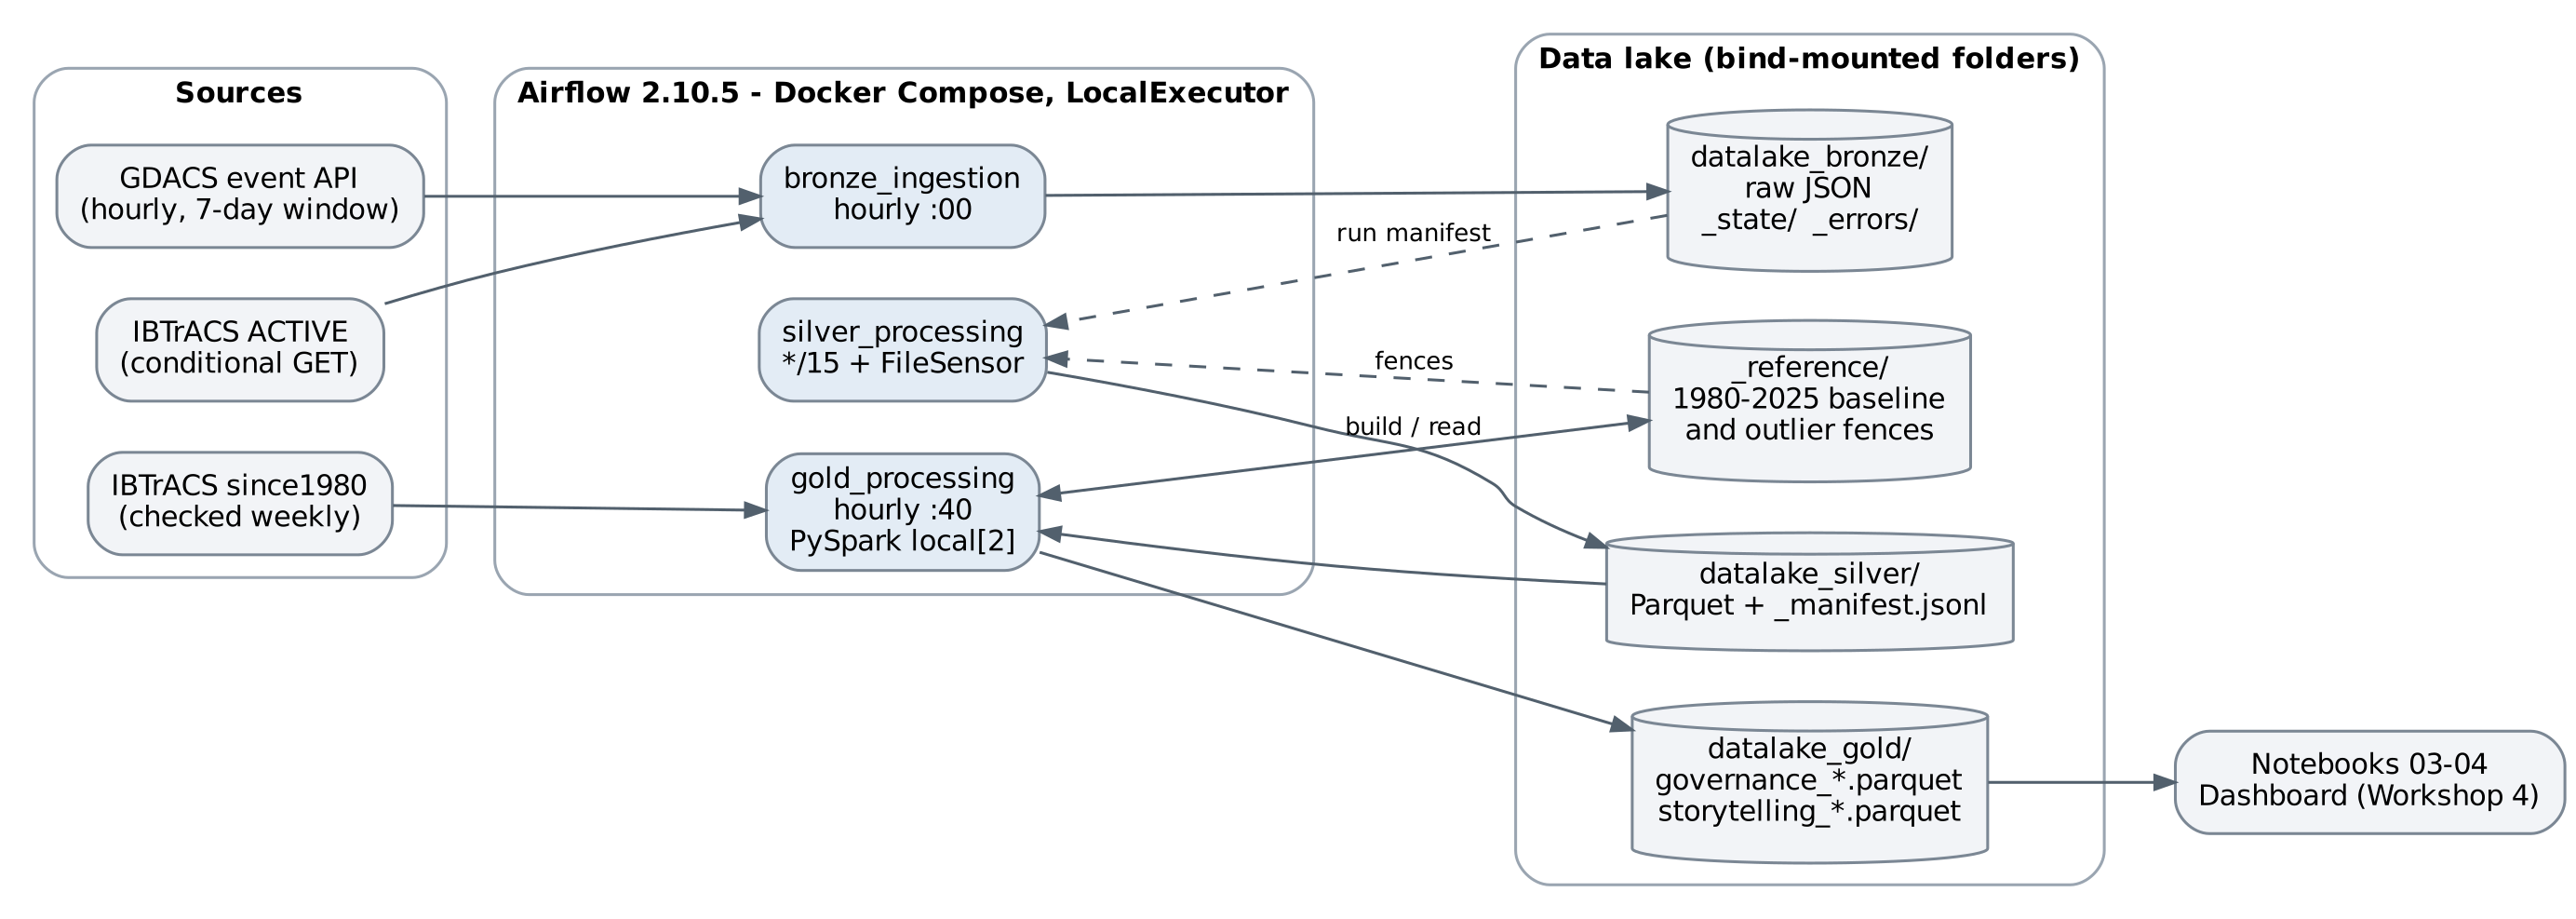
\includegraphics[width=0.92\textwidth]{arch.png}
\caption{Three-layer pipeline after Workshop~3. Dashed arrows are signals rather than data copies: the Bronze run manifest that wakes the Silver FileSensor, and the climatological fences that Silver reads from the reference built by Gold.}
\label{fig:arch}
\end{figure*}

The Airflow image now contains OpenJDK~17 and PySpark~3.5.4, installed against the official Airflow~2.10.5 constraints so that no Airflow dependency is upgraded. The build checks that PySpark imports and that Java runs; it took 7~min on the deployment laptop (Docker limited to 11.5~GB, 12~CPUs).

\section{Data-Quality Findings}\label{sec:findings}

The audit read only metadata and data already in the lake: Bronze envelopes, error bodies, \code{\_manifest.jsonl} and the Silver Parquet files. Runs made before the improvements are labeled Workshop~2; runs that write the new ingestion log are labeled Workshop~3. Table~\ref{tab:findings} summarizes the nine findings.

\begin{table*}[t]
\caption{Data-Quality Findings, Improvements and Monitoring KPIs}\label{tab:findings}
\centering\footnotesize
\begin{tabularx}{\textwidth}{@{}c L{4.2cm} Y L{4.0cm} c@{}}
\toprule
\# & Finding & Evidence (Workshop~2 data) & Improvement & KPI\\
\midrule
F1 & GDACS returns HTTP~400 ``Execution Timeout Expired'' & 5 failed hourly runs between 17~Nov 23:00 and 18~Nov 03:00~UTC, 31.8--38.8~s each; error bodies left in \code{\_staging/} & short 400 bodies with ``timeout'' retried (4, 8, 16~s); bodies moved to \code{\_errors/}; every attempt logged & C3\\
F2 & IBTrACS ACTIVE stored every hour although unchanged & 13 files, only 2 distinct contents (ETags of 15 and 17~Nov); 11 redundant files, 6.36 of 7.53~MB; about 13.7~MB/day & conditional GET with stored ETag and Last-Modified, plus SHA-256 check; no file when unchanged & E1, E2\\
F3 & File timestamps earlier than the ingestion & scheduled runs named with the start of the data interval: median delay 60--64~min, run \code{\ldots\_220000} ingested at 23:53 & scheduled runs named with \code{data\_interval\_end}, manual runs with the trigger time & T1\\
F4 & Empty Silver files & 7 of 12 Silver runs wrote 0-row files of 18.9~kB & no file when nothing is new; run kept in the manifest & F4\\
F5 & Silver file named before its input & 3 of 12 runs (e.g. Silver \code{\ldots\_020000} processed Bronze \code{\ldots\_021437}) & Silver takes the later of its run time and its newest Bronze run & F5\\
F6 & Batch IQR flagged a real typhoon peak & batch fences [5.3, 71.3]~kt: 16 flags, every CEMPAKA fix of 74--93~kt; same storm with 0 flags in later batches & fences from 1980--2025 climatology, applied to the 6-hourly wind change & V4, V5, V9\\
F7 & Structural and real nulls mixed & GDACS has no current wind, pressure or motion (100\% null by design); real gaps: pressure 3.0\%, names 9.5\%; all fixes provisional & null rate per source and field & C1, V7\\
F8 & Sources disagree and are not equally fresh & XAVIER: GDACS peak 130~kt vs IBTrACS 99~kt, GDACS 78~h ahead & both kept, with the lead time & K1--K3, T3\\
F9 & Name formats & GDACS names average 25.5 characters (\code{Tropical Cyclone XAVIER-26}) and 5.5 after normalization & normalization measured & K4, K5\\
\bottomrule
\end{tabularx}
\end{table*}

Two findings deserve comment. F2 is shown in Fig.~\ref{fig:f2}: grey bars are Bronze files identical to the previous one. At 24 runs per day the behavior of Workshop~2 would have stored about 5~GB of duplicates per year, and each copy also forced the Silver layer to deduplicate 142 rows again (1,585 of the 1,901 input rows of Workshop~2, 83\%, were already in Silver). F6 is shown in Fig.~\ref{fig:f6}: the Workshop~2 rule computed the interquartile range of the wind \emph{level} inside each batch \cite{tukey}, so a strong but genuine storm became an ``outlier'' only because the other storms of the batch were weak.

\begin{figure}[t]
\centering
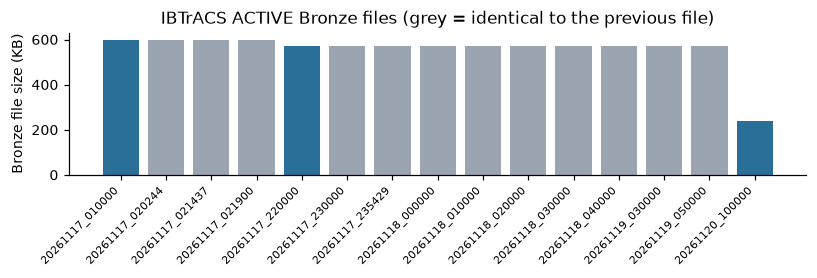
\includegraphics[width=\columnwidth]{f2_ibtracs_redundant.png}
\caption{Size of every IBTrACS ACTIVE Bronze file. Grey bars are byte-identical to the previous file. The last bar is the new NCEI release of 20~Nov 03:12~GMT, the only download after the bootstrap run of Workshop~3.}
\label{fig:f2}
\end{figure}

\begin{figure*}[t]
\centering
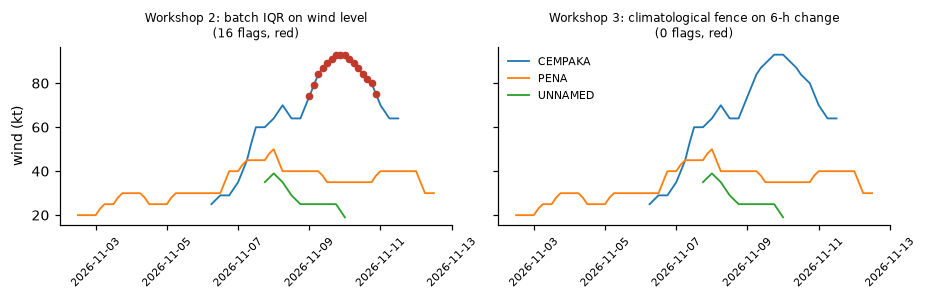
\includegraphics[width=0.78\textwidth]{f6_outlier_rule.png}
\caption{Wind outliers in the Bronze batch of 17~Nov 01:00~UTC. Left: batch IQR on the wind level (16 flags, all at the peak of CEMPAKA). Right: climatological 3$\cdot$IQR fence on the 6-hourly wind change (no flags in this batch).}
\label{fig:f6}
\end{figure*}

\section{Pipeline Improvements}\label{sec:improve}

The improvements changed the code of Bronze and Silver but not their contracts: Bronze still stores records exactly as published, and the Silver schema keeps its 38 fields. Only the meaning of the two statistical flags changed, and both are excluded from the record hash, so the new rule does not create false revisions. Table~\ref{tab:beforeafter} compares the two versions on the same data lake.

\begin{table}[t]
\caption{Before and After, Measured on the Same Data Lake}\label{tab:beforeafter}
\centering\footnotesize
\begin{tabularx}{\columnwidth}{@{}Y L{2.0cm} L{2.0cm}@{}}
\toprule
Measure & Workshop~2 & Workshop~3\\
\midrule
GDACS extraction attempts failed & 5 of 18 & 0 of 17\\
IBTrACS checks that stored a file & 13 of 13 & 2 of 17\\
Redundant IBTrACS volume & 6.36~MB & 0.57~MB\textsuperscript{a}\\
Median timestamp-to-ingestion delay & 60--64~min & 1.2~min\textsuperscript{b}\\
Empty Silver files written & 7 of 12 & 0 of 15\\
Silver named before its input & 3 of 12 & 0 of 10\textsuperscript{c}\\
Wind flags, 17~Nov 01:00 batch & 16 & 0\\
\bottomrule
\end{tabularx}\\[2pt]
\parbox{\columnwidth}{\scriptsize \textsuperscript{a}The bootstrap download of the first Workshop~3 run (no stored validators yet). \textsuperscript{b}Two runs reach 17--18~h because Airflow created them just before the laptop was shut down and executed them at restart. \textsuperscript{c}Runs after the fix of 20~Nov 01:30~UTC; 3 of the 5 earlier Workshop~3 runs were still named before their input.}
\end{table}

\subsubsection{Conditional GET} The IBTrACS file is requested with \code{If-None-Match} and \code{If-Modified-Since}; the validators are written to \code{\_state/} only after the Bronze file is safely stored. Between 19 and 21~Nov the server answered ``not modified'' 15 times, and the pipeline downloaded once more only when NCEI published a new release (58 records, 20~Nov 03:12~GMT). A run without an IBTrACS file is still complete: the Bronze signal task reads the ingestion log to know which files to expect.

\subsubsection{Transient errors} GDACS reports a database timeout with a 400 code, which an HTTP client normally treats as a client error. The client now retries a short 400 body that contains ``timeout''. No timeout occurred after the change, so the retry path is covered by a unit test that uses the real body of 18~Nov rather than by production evidence.

\subsubsection{Run timestamps} Airflow's \code{logical\_date} is the start of the data interval \cite{airflow}. Bronze, Silver and Gold now share one helper that returns \code{data\_interval\_end} for scheduled runs and the trigger time for manual runs (Fig.~\ref{fig:f3}). A second fix was needed in Silver: its FileSensor can wait up to 14~min, so a Silver run started at 21:45 could process the Bronze run of 22:00. The Silver file now takes the later of the two moments.

\begin{figure}[t]
\centering
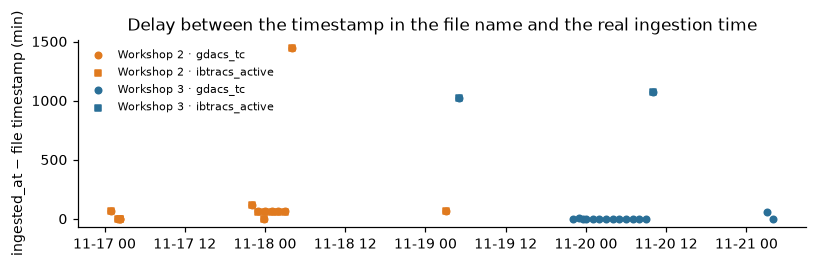
\includegraphics[width=\columnwidth]{f3_timestamp_delay.png}
\caption{Delay between the timestamp in the file name and the real ingestion time. Orange: Workshop~2 (about 1~h for scheduled runs). Blue: Workshop~3 (about 1~min). The two isolated blue points are runs executed after the laptop was restarted.}
\label{fig:f3}
\end{figure}

\subsubsection{Climatological outlier fences} The reference archive (Section~\ref{sec:gold}) gives 132,850 six-hourly wind changes from 5,019 storms. With $Q_1=0$ and $Q_3=5$~kt, the 3$\cdot$IQR fence is $[-15, +20]$~kt per 6~h; for translation speed the mean is 10.0~kt and the standard deviation 6.7~kt, so $|z|>3$ starts at 30.0~kt. The fences no longer move with the batch. The wind rule now flags only unusually fast changes; for scale, rapid intensification is usually defined as at least 30~kt in 24~h \cite{kaplan}. CEMPAKA still receives four speed flags at 34--36~kt, which is correct: it was moving fast while leaving the tropics.

\subsubsection{Other changes} Silver writes no file for a batch without new or changed records; the manifest records the run with \code{silver\_file = null}. Gold reads only the latest version of each \code{event\_id}, because GDACS edits records in place: episode~13 of AKVAN changed its \code{datemodified} nine times, giving 16 revisions among 231 Silver rows.

\section{Gold Layer}\label{sec:gold}

The DAG \code{gold\_processing} runs every hour at minute 40, after the Bronze run of minute~0 has reached Silver. Its six tasks are \code{run\_timestamp}, \code{check\_silver\_inputs} (skips the run if Silver is empty), \code{ensure\_reference}, \code{build\_governance}, \code{build\_storytelling} and \code{verify\_gold}, which reads both files back, checks their schemas and deletes Gold files older than 14~days.

\subsection{PySpark in Local Mode}
Each Spark task starts a session with \code{local[2]}, a 2~GB driver, four shuffle partitions, the UI disabled and the session time zone set to UTC \cite{pyspark}. The input is read exactly as the guide asks, \code{spark.read.parquet("datalake\_silver/")}. Spark skips every path that begins with an underscore or a dot, so \code{\_manifest.jsonl}, \code{\_rejected/} and \code{\_reference/} are not mixed with the data. A window function keeps the latest version of each event. Spark writes a folder of part files, while the guide requires one file per table; the result is therefore coalesced to one partition, written to a temporary folder whose name starts with an underscore, and its single part file is renamed atomically to \code{governance\_YYYYMMDD\_HHMMSS.parquet} or \code{storytelling\_YYYYMMDD\_HHMMSS.parquet}. Timestamps are written as microseconds, so Pandas and Spark read them alike.

The current data are small (231 Silver rows), so Spark does not make Gold faster than Pandas would. It is used because the course requires it and because the same code will scale with the lake and with the historical archive, which already has 312,416 rows \cite{zaharia}.

\subsection{Historical Reference}
The analogs need the IBTrACS v04r01 \code{since1980} archive \cite{ibtracs,knapp}. It is 145~MB, so it does not go through the hourly flow. The task \code{ensure\_reference} checks it at most once a week with a conditional GET; when NCEI publishes a new file it reads the CSV in chunks of 50,000 rows, applies the same conforming rules as Silver (USA wind first, then WMO wind; longitudes in $[-180,180)$; spur flag), and writes \code{datalake\_silver/\_reference/ibtracs\_since1980.parquet} together with the outlier fences. The first build downloaded the archive in 14~s and processed 312,416 fixes of 5,019 storms in 23~s.

\subsection{Tidy Output Tables}
Both Gold tables are long: one row per KPI value or per story fact, with a \code{gold\_run\_ts} column. A new KPI or a new story section never changes the file schema, and the history of any metric can be read across runs. In the notebook, Spark read all 18 governance files of the week at once to show how the KPI statuses changed from run to run.

\section{Governance KPIs}\label{sec:gov}

The KPIs follow the data-quality dimensions of DAMA-DMBOK and ISO/IEC~25012 \cite{dama,iso25012,wang}. Table~\ref{tab:kpis} lists the 37 KPI definitions by dimension. Each one has a unit, a target when one makes sense, and a status: \code{ok}, \code{warn}, \code{fail}, \code{info} (descriptive) or \code{n/a}. Besides Silver, the governance task reads metadata only (Bronze envelope headers, the ingestion logs, the error folder, the Silver manifest and Parquet footers), and every aggregation runs in Spark.

\begin{table}[t]
\caption{Governance KPI Catalogue}\label{tab:kpis}
\centering\footnotesize
\begin{tabularx}{\columnwidth}{@{}L{1.55cm} Y c@{}}
\toprule
Dimension & KPIs (examples) & Story\\
\midrule
Completeness & C1 null rate per source and field (target 0\% for required fields); C2 hourly slots covered per day; C3 extraction success rate & US-04\\
Uniqueness & U1 cross-batch duplicates; U2 within-batch duplicates; U3 revisions; U4 older versions & US-07\\
Validity & V1 rejected rows; V2 values out of bounds; V3--V5 missing wind, wind-change and speed outliers; V6 derived motion; V7 provisional; V8 spur; V9 fence basis & US-07\\
Conformity & F1 schema match; F2 file naming; F3 lineage metadata; F4 empty files; F5 file named before its input & --\\
Timeliness & T1 delay to ingestion; T2 Bronze-to-Silver latency; T3 age of newest observation; T4 hours since last file & US-04\\
Consistency & K1 GDACS minus IBTrACS peak; K2 GDACS lead time; K3 storms in both sources; K4 name changes; K5 unnamed & US-04\\
Efficiency, volume & E1 identical consecutive files; E2 ``not modified'' answers; E3--E5 records per day and per source & --\\
\bottomrule
\end{tabularx}
\end{table}

The sample file \code{governance\_20261121\_040036.parquet} holds 149 KPI values: 59 \code{ok}, 1 \code{warn}, 16 \code{fail} and 73 \code{info} (Fig.~\ref{fig:kpi}). The failures are real and explainable. Ten are C2 values between 4\% and 46\%: the pipeline runs on a laptop that was on only part of each day, so most hourly slots have no run. The KPI measures availability of the whole system and should stay strict. C3 is 85.3\% because it still counts the five GDACS timeouts of F1. E1, F4, F5 and T1 also carry history from Workshop~2: the file counts never decrease, so these KPIs will improve only as new runs dilute the old ones. This is a deliberate choice; a KPI that silently forgets past problems is less useful for governance. The only warning, T3, says that the newest IBTrACS fix was 40~h old, which matches the publication rhythm of the ACTIVE file.

\begin{figure}[t]
\centering
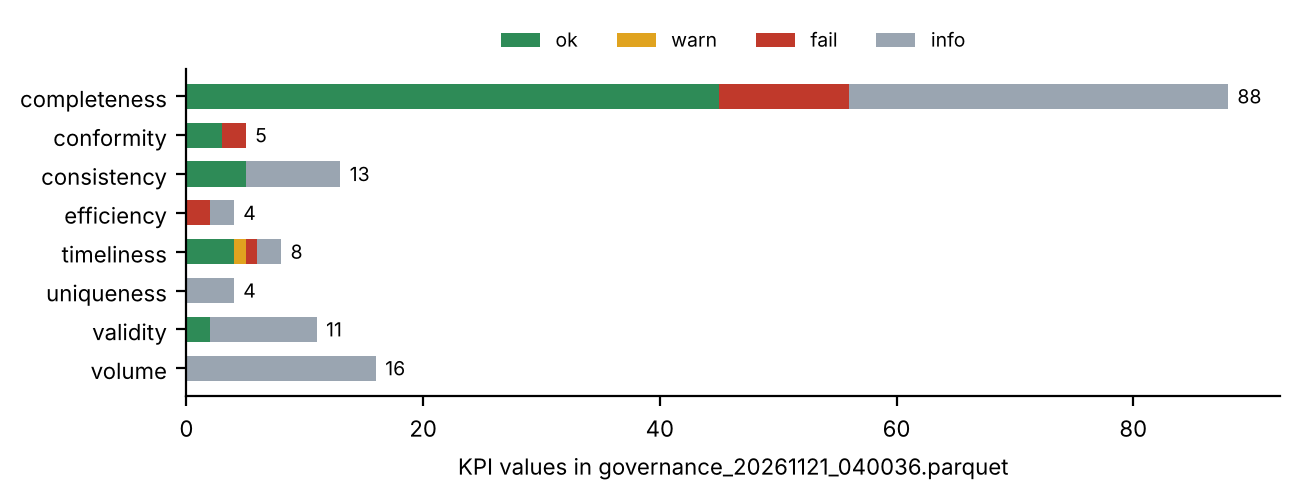
\includegraphics[width=\columnwidth]{kpi_status.png}
\caption{Status of the 149 KPI values in the sample governance file, grouped by quality dimension. Completeness dominates because C1 gives one value per source and field.}
\label{fig:kpi}
\end{figure}

The KPIs also proved useful for the data themselves. On 20~Nov the consistency KPI K1 marked XAVIER as \code{fail}: GDACS reported 130~kt and IBTrACS 99~kt. After NCEI published the new ACTIVE file, the difference fell to 2~kt (130 vs. 128~kt) and the GDACS lead from 78~h to 36~h. The two sources did not disagree; the best-track file was old, and the KPI made that visible.

\section{Storytelling}\label{sec:story}

\subsection{Sections and User Stories}
The storytelling table has ten sections, each tied to the user stories of Workshop~1 (Table~\ref{tab:sections}). A storm is ``current'' when its last best-track fix is less than seven days older than the newest fix in Silver.

\begin{table}[t]
\caption{Storytelling Sections and User Stories}\label{tab:sections}
\centering\footnotesize
\begin{tabularx}{\columnwidth}{@{}L{2.1cm} c Y@{}}
\toprule
Section & Story & Content\\
\midrule
current\_status & US-01, 06 & last fix, wind, category, motion, GDACS alert\\
whats\_new & US-02 & new and revised records in 24~h\\
intensity\_track & US-05 & wind and pressure of every fix\\
analogs & US-03 & top-5 analogs with every SAS term\\
analog\_outcomes & US-03, 05 & analog wind 24--72~h later, landfall\\
analog\_tracks & US-05 & aligned tracks for the overlay plot\\
gdacs\_alerts & US-01, 02 & alert level and score per episode\\
source\_comparison & US-04 & peak difference and GDACS lead\\
basin\_climatology & US-08 & basin statistics and percentile\\
narrative & all & one paragraph per storm\\
\bottomrule
\end{tabularx}
\end{table}

\subsection{Storm Analog Similarity}
The analog idea is old in meteorology: look for past states of the atmosphere that resemble the present one \cite{lorenz}. Our indicator, defined in Workshop~1, compares the last 48~h of a current storm, at 00, 06, 12 and 18~UTC, with every 48-h window of every storm of the same basin since 1980:
\begin{equation}
D=\tfrac14\Bigl(\tfrac{\bar d_{\mathrm{track}}}{250\,\mathrm{km}}+\tfrac{\overline{|\Delta V|}}{15\,\mathrm{kt}}+\tfrac{\overline{|\Delta\theta|}}{45^\circ}+\tfrac{|\Delta\mathrm{doy}|}{30\,\mathrm{d}}\Bigr),\quad \mathrm{SAS}=100\,e^{-D}.
\end{equation}
Candidates must have a final (\code{main}) track, a six-hourly fix within 300~km of the current position, and must have ended at least 15~days before; the best window of each candidate is kept and the five lowest $D$ are reported. A term that cannot be computed counts as one reference unit (Section~\ref{sec:challenges}). The Spark version is a set of joins and window functions; a separate Pandas version computes the same indicator with loops, and a test checks that both give the same SAS to nine significant digits.

\subsection{Results}
The sample \code{storytelling\_20261121\_040036.parquet} has 1,003 rows for three current storms. Table~\ref{tab:analogs} shows the best analogs; the narratives are built only from those rows and end with the same sentence: analogs describe resemblance with past storms, they are not a forecast.

\begin{table}[t]
\caption{Best Analogs in the Sample Storytelling File}\label{tab:analogs}
\centering\footnotesize
\begin{tabularx}{\columnwidth}{@{}l c Y c c@{}}
\toprule
Storm & Wind & Best analog (SAS) & Track & $|\Delta V|$\\
\midrule
XAVIER, SP & 105~kt & MARTIN 1998 (29, low) & 146~km & 48~kt\\
AKVAN, NI & 35~kt & unnamed 2002 (66, moderate) & 213~km & 1~kt\\
PENA, EP & 30~kt & unnamed 1997 (55, moderate) & 169~km & 11~kt\\
\bottomrule
\end{tabularx}
\end{table}

\emph{XAVIER} (Fig.~\ref{fig:xavier}) is the clearest case. At its last fix (19~Nov 12:00~UTC, 10.6\textdegree{}S, 163.1\textdegree{}W) it had 105~kt, a Category~3 on one-minute winds \cite{sshs}, after a peak of 128~kt, and it was almost stationary. Its peak is above the lifetime maximum of 95\% of South Pacific storms since 1980. The best analog scores only 29, and the other four between 9 and 18: the archive has no storm that was this strong in this place at this time of year. Here a low SAS is itself the story.

\emph{AKVAN} (Fig.~\ref{fig:akvan}) is a weak storm in the Bay of Bengal that turned north at 16\textdegree{}N, 85.3\textdegree{}E. Its five analogs have SAS between 52 and 66. In the 48~h after their matching point, four of them weakened (median $-10$~kt) and four reached land within 72~h. This is the kind of context US-03 asks for: what similar storms did next, given as history and not as a prediction.

\begin{figure*}[t]
\centering
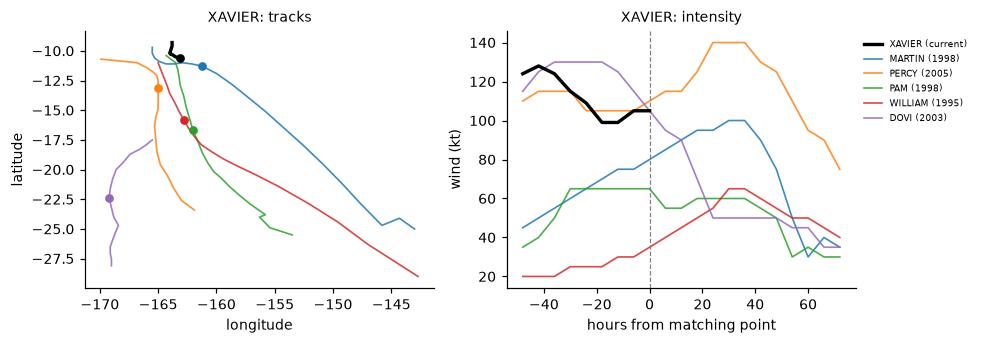
\includegraphics[width=0.85\textwidth]{g3_analogs_XAVIER.png}
\caption{XAVIER (black) and its five analogs. Left: tracks, with the matching points as dots. Right: wind against hours from the matching point; the analogs continue 72~h beyond it. All analogs were much weaker than XAVIER at the matching point, hence the low SAS.}
\label{fig:xavier}
\end{figure*}

\begin{figure*}[t]
\centering
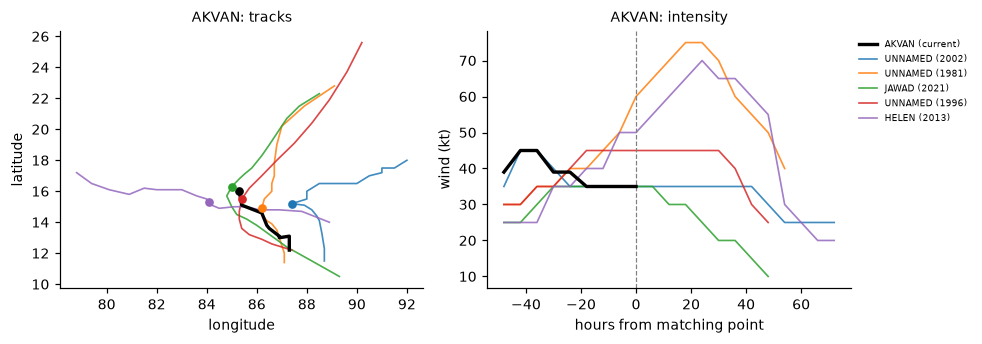
\includegraphics[width=0.85\textwidth]{g3_analogs_AKVAN.png}
\caption{AKVAN (black) and its five analogs in the Bay of Bengal. Most analogs moved north toward the coast and weakened after landfall.}
\label{fig:akvan}
\end{figure*}

\section{Challenges and Decisions}\label{sec:challenges}

\subsubsection{Out of memory in Spark} The first three storytelling runs failed after about 3~min with \code{java.lang.OutOfMemoryError: Java heap space} (Fig.~\ref{fig:runs}). The data were tiny; the problem was the query plan. The function that turns wide rows into tidy rows built one \code{select} per metric and joined them with \code{union}, and every \code{select} repeated the whole chain of analog joins. Spark then wrote the text of a huge plan for its event log and filled the 2~GB driver. The fix packs all metrics of a section into an array of structs that is exploded once, materializes each section with \code{localCheckpoint}, and caps \code{spark.sql.maxPlanStringLength}. The task now finishes in about 2~min.

\begin{figure}[t]
\centering
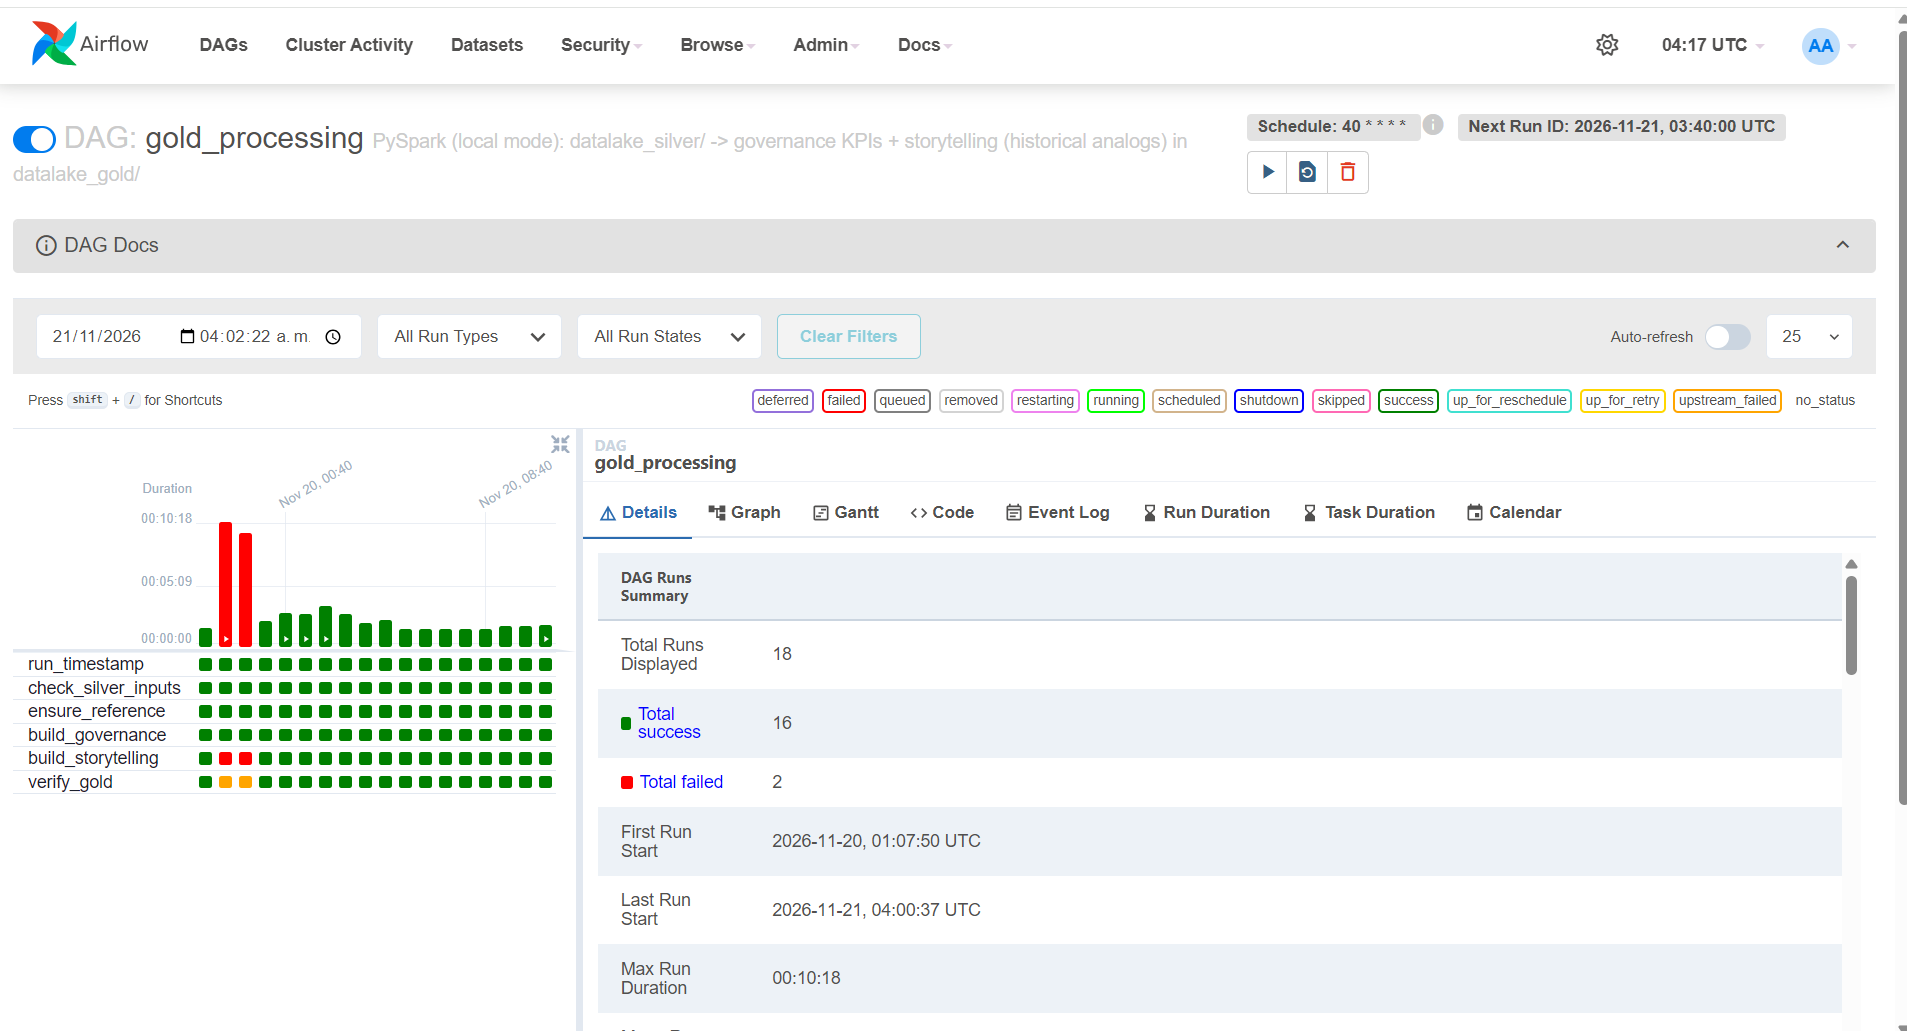
\includegraphics[width=\columnwidth]{gold_runs_grid.png}
\caption{Grid view of \code{gold\_processing} on 21~Nov: 18 runs: two stopped by the memory error in \code{build\_storytelling} (red) and 16 successful runs after the fix.}
\label{fig:runs}
\end{figure}

\subsubsection{Analogs without wind} In the first successful run, AKVAN's best analog was a 1988 storm with SAS 77, ``high'', but no wind difference. Old North Indian records often have no wind in IBTrACS, and the first version dropped a missing term and rescaled the other weights, so an analog with \emph{unknown} intensity looked closer than one with a known intensity. A missing wind or heading term now counts as one reference unit (15~kt or 45\textdegree), and the formula keeps its four terms as defined in Workshop~1.

\subsubsection{Narrative with missing outcomes} CEMPAKA's analogs all ended within 48~h of their matching point, and the narrative printed ``None of 5 analogs intensified''. The summary now counts the analogs still tracked at 48~h and says so when there are none.

\subsubsection{A threshold set too strictly} The within-batch duplicate KPI first had a target of 0\%, but duplicates inside one batch are expected when a Silver run claims several Bronze runs with the same content. It became descriptive.

\subsubsection{Laptop as a server} Every fix was tested inside the Airflow container: 45 tests pass, including four Spark tests on a small lake built from recorded responses. The remaining limitation is the host: the stack runs only while the laptop is on, which explains the C2 values and the two late runs of Table~\ref{tab:beforeafter}.

\section{Conclusion}
The three layers now run end to end. The audit of real data changed more than expected: one source fails in a way HTTP clients do not expect, another publishes far less often than we polled it, and our own outlier rule was wrong. The Gold layer turns those lessons into KPIs that can be followed run by run, and it delivers the comparison promised in Workshop~1 for every current storm. Workshop~4 will build the dashboard on top of the two Gold tables.

\balance
\begin{thebibliography}{20}
\footnotesize
\setlength{\itemsep}{1pt}
\bibitem{ws3} C.~A. Sierra, ``Workshop No.~3: Silver-to-Gold pipeline, governance KPIs, and storytelling definition,'' Data Analysis Programming, Universidad Distrital Francisco José de Caldas, Bogotá, Colombia, 2026.
\bibitem{ws1rep} O.~Peña, R.~López, and B.~Ramírez, ``TC-Analog Monitor: Hazard definition, source validation and data contract,'' Workshop~1 report, Universidad Distrital Francisco José de Caldas, Nov. 2026.
\bibitem{ws2rep} O.~Peña, R.~López, and B.~Ramírez, ``TC-Analog Monitor: Technical architecture and Bronze/Silver pipeline for tropical cyclone data,'' Workshop~2 report, Universidad Distrital Francisco José de Caldas, Nov. 2026.
\bibitem{airflow} The Apache Software Foundation, ``Apache Airflow 2.10 documentation: DAG runs, data intervals and sensors.'' [Online]. Available: \url{https://airflow.apache.org/docs/apache-airflow/2.10.5/}
\bibitem{pyspark} The Apache Software Foundation, ``PySpark 3.5 documentation: Spark SQL, DataFrames and configuration.'' [Online]. Available: \url{https://spark.apache.org/docs/3.5.4/api/python/}
\bibitem{zaharia} M.~Zaharia \emph{et al.}, ``Apache Spark: A unified engine for big data processing,'' \emph{Commun. ACM}, vol.~59, no.~11, pp.~56--65, 2016.
\bibitem{dama} DAMA International, \emph{DAMA-DMBOK: Data Management Body of Knowledge}, 2nd~ed. Basking Ridge, NJ, USA: Technics Publications, 2017.
\bibitem{iso25012} \emph{Software Engineering \textemdash{} Software Product Quality Requirements and Evaluation (SQuaRE) \textemdash{} Data Quality Model}, ISO/IEC 25012:2008.
\bibitem{wang} R.~Y. Wang and D.~M. Strong, ``Beyond accuracy: What data quality means to data consumers,'' \emph{J. Manage. Inf. Syst.}, vol.~12, no.~4, pp.~5--33, 1996.
\bibitem{tukey} J.~W. Tukey, \emph{Exploratory Data Analysis}. Reading, MA, USA: Addison-Wesley, 1977.
\bibitem{ibtracs} J.~Gahtan \emph{et al.}, ``International Best Track Archive for Climate Stewardship (IBTrACS) Project, Version 4.01,'' NOAA NCEI, 2024, doi: 10.25921/82ty-9e16.
\bibitem{knapp} K.~R. Knapp, M.~C. Kruk, D.~H. Levinson, H.~J. Diamond, and C.~J. Neumann, ``The International Best Track Archive for Climate Stewardship (IBTrACS): Unifying tropical cyclone data,'' \emph{Bull. Amer. Meteor. Soc.}, vol.~91, no.~3, pp.~363--376, 2010.
\bibitem{gdacs} Global Disaster Alert and Coordination System, ``GDACS API quick start,'' European Commission Joint Research Centre and UN OCHA, 2025.
\bibitem{lorenz} E.~N. Lorenz, ``Atmospheric predictability as revealed by naturally occurring analogues,'' \emph{J. Atmos. Sci.}, vol.~26, no.~4, pp.~636--646, 1969.
\bibitem{kaplan} J.~Kaplan and M.~DeMaria, ``Large-scale characteristics of rapidly intensifying tropical cyclones in the North Atlantic basin,'' \emph{Weather Forecast.}, vol.~18, no.~6, pp.~1093--1108, 2003.
\bibitem{sshs} T.~Schott \emph{et al.}, ``The Saffir-Simpson hurricane wind scale,'' NOAA National Hurricane Center, 2012.
\end{thebibliography}

\end{document}
